\section{Background}

\subsection{Cothority framework}

\paragraph{}

The apparition of BlockChain technologies has allowed easy and scalable collaboration between users and decentralisation of information. In that scope, \textit{Cothority} allows to form \textit{Collective Authorities} that run decentralised and distributed protocols on a set of \textit{Cothority Servers}, a.k.a \textit{Conodes}\footnote{\url{https://github.com/dedis/cothority}}.

\paragraph{}

\textit{Cothority} is implemented using a number of protocols designed to overcome the basic challenges of running algorithms in a decentralised way. They implement most of the consensus and cryptographic functions needed by the framework to properly work.

\paragraph{}

DEDIS has also implemented a number of applications on this framework, notably \textit{Proof of Personhood}\footnote{\url{https://github.com/dedis/cothority/tree/master/pop}} and \textit{ByzCoin}\footnote{\url{https://github.com/dedis/cothority/tree/master/byzcoin}}. This project concerning mostly the second one, this report will not introduce \textit{POP}.

\subsubsection{ByzCoin}

\paragraph{}

\textit{ByzCoin} is an implementation of the \textit{OmniLedger} protocol\footnote{\url{https://eprint.iacr.org/2017/406.pdf}} designed by DEDIS lab at EPFL. It is a coin based on a \textit{SkipChain}\footnote{\url{https://github.com/dedis/cothority/tree/master/skipchain}} that is designed to work on a \textit{Cothority}. Its operation is better described by \href{https://raw.githubusercontent.com/dedis/cothority/master/byzcoin/ByzCoin.png}{this picture (click)}.

\paragraph{}

The creation of a \textit{ByzCoin} instance was already implemented at the beginning of the project. Based on a roster (its \textit{Collective Authority}), it is created with a \textit{Genesis DARC} and an \textit{Admin Identity}. One of the goals of this project was to be able to create and manage other \textit{DARC} than the \textit{Genesis} one, for users who are not necessarily the Admin.

\paragraph{}

In order for a client to be able to interact with a \textit{ByzCoin} instance, it needs to know its configuration. The content of the \textit{Config} object may differ from implementation to implementation, but in any case it must contain:

\begin{itemize}
    \item The \textit{ByzCoin} instance ID
    \item The \textit{Roster}, which is the set of \textit{Conodes} on which the \textit{ByzCoin} is deployed
\end{itemize}

It may also contain:

\begin{itemize}
    \item The \textit{Genesis DARC}
    \item The Admin identity (public key)
\end{itemize}

\subsubsection{DARC}
\label{subsection212}

\paragraph{}

One of the most important components of \textit{ByzCoin} is \textit{Distributed Access Rights Control}, a.k.a \textit{DARC}. These structures allow a decentralised management of the access rights in the different instances of \textit{ByzCoin}.

\paragraph{}

Each \textit{DARC} holds the following information:
\begin{itemize}
    \item Description (String)
    \item Version (Integer, the number of time its been evolved. It is sometimes also called Depth)
    \item ID (a SHA-256\footnote{\url{https://csrc.nist.gov/groups/ST/toolkit/secure_hashing.html}} digest of its own content)
    \item BaseID (the ID of its first version)
    \item PrevID (the ID of the \textit{DARC} from which it was spawned)
    \item Rules (explained hereafter)
    \item Signatures (a set of signatures)
\end{itemize}

\paragraph{}

The rules are a set of action-expression pairs that regulate what can be done from a given \textit{DARC}. While the action describes the instruction that can be signed, the expression describes using logical expressions which \textit{DARC} or users must/can sign in order for the transaction to be valid.

\paragraph{}

Most used actions for \textit{DARC} management include but are not limited to:
\begin{itemize}
    \item \textit{spawn:darc}
    \item \textit{invoke:evolve}
    \item \textit{\_sign}
\end{itemize}

\paragraph{}

Expressions use ED25519\footnote{\url{https://ed25519.cr.yp.to/}} keys to identify the users. Using logical expressions allows them to require multiple signatures, or one signature amongst a set.

\paragraph{}

In order to add a \textit{DARC} to a \textit{ByzCoin} instance, one must \textit{spawn} it. A user who wants to spawn a \textit{DARC} B first needs to have a \textit{DARC} A on which he has the right to perform the action \textit{spawn:darc}: it will be expressed in this report as spawning B \textit{from} A.

\paragraph{}

\textit{DARC} can have what is called an \textit{owner}. The owner is a user having an exclusive access right on actions \textit{\_sign} and \textit{invoke:evolve}. As such, he is free to sign with his \textit{DARC} and evolve it to manage it as he sees fit. At spawn, \textit{DARC} are usually created with an owner and comprise only those two rules, both linked with an expression composed only of the public key of the owner.

\paragraph{}

As \textit{DARC} are part of the \textit{SkipChain} blocks, they are immutable objetcs. In order to edit their settings, any user having the right to do so (through the \textit{invoke:evolve} action) can \textit{evolve} a \textit{DARC}. 

\paragraph{}

To evolve \textit{DARC} A, the client first creates a copy - B. It then makes the changes the user desires on B, and increments the version number. As the content of the \textit{DARC} will have changed, B will have a different ID from A (as it is a SHA-256 digest of the information it holds). However, A and B will still keep the same \textit{BaseID}, which is the ID of their first ancestor, and will be identified by it. After having made these changes, the client puts B inside an \textit{Instruction}, which it sends to \textit{ByzCoin} through a \textit{Transaction}. The \textit{Cothority} then \textit{spawns} B and will return it when asked for the \textit{BaseID} of both A and B.

\subsection{BC Admin CLI}

\paragraph{}

The BC Admin CLI\footnote{\url{https://github.com/dedis/cothority/tree/master/byzcoin/bcadmin}} is implemented in Go using the CLI V1 package from \textit{gopkg.in}\footnote{\url{https://github.com/urfave/cli/tree/v1.20.0}}. Some basic functionalities were already implemented at the start of the project:
\begin{itemize}
    \item Creating new \textit{ByzCoin} based on a given roster
    \item Evolving the \textit{Genesis DARC} to add a rule
    \item Showing the \textit{Genesis DARC} in the terminal
\end{itemize}

\paragraph{}
But these are not enough to correctly manage a \textit{ByzCoin} and its access rights. The first part of the project thus was implementing some new functionalities to it, as will be described in \hyperref[section4]{section 4}.

\subsection{PopCoins}

\paragraph{}

\textit{PopCoins} is a \textit{NativeScript} cross-platform mobile application developed by DEDIS lab\footnote{\url{https://github.com/dedis/popcoins}} in order to propose \textit{Cothority} applications in a simple, user-friendly way.

\begin{figure}[!h]
    \centering
    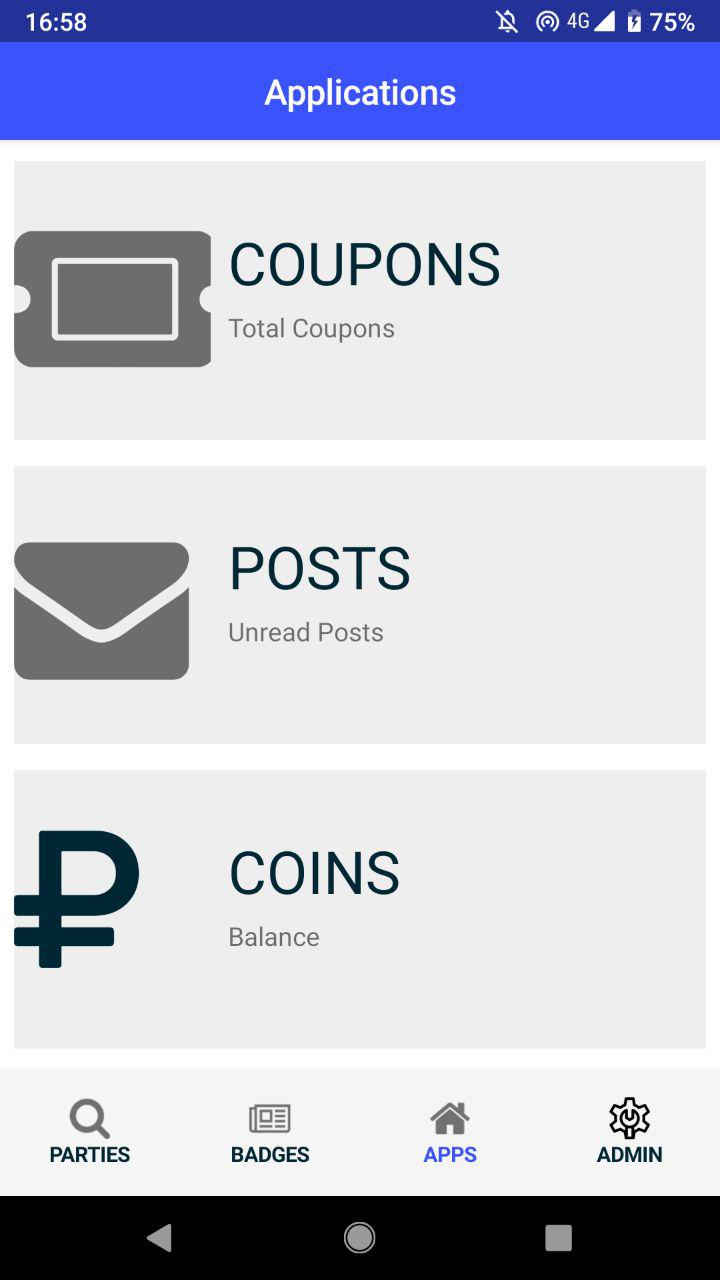
\includegraphics[height=0.8\linewidth]{Illustrations/screen_mainmenu.jpg}
    \caption{\textit{PopCoins} main menu}
\end{figure}

\paragraph{}

\textit{PopCoins}, at the beginning of the project, implemented features mainly linked with the \textit{POP} application. As such, the features implemented during the course of this project did not modify the already implemented functionalities, as they were only remotely linked. It however reuses a lot of tools, such as those for the management of the \textit{Conodes}, or the different clients and sockets linked with the \textit{Cothority} services.

\subsubsection{NativeScript}

\paragraph{}

\textit{NativeScript}\footnote{\url{https://www.nativescript.org/}} is a framework that allows to develop native cross-platform applications, compatible with both iOS and Android. It uses \textit{JavaScript} for application logic, and a XML-CSS combination for the User Interface (UI). It also offers the opportunity to use native iOS and Android APIs through different bindings: this possibility has however not had to be used during this project

\subsubsection{Application UI}

\paragraph{}

The UI of the application is built around a first page describing the apps currently available. This is the most user-friendly area, where a non-initiated person should feel at ease. As such, details about \textit{DARC} being quite technical, they have not been implemented in this part of the application.

\paragraph{}

An other part of the application is the Admin menu. It contains settings about coupons, new parties (both used for \textit{POP}), and \textit{conodes}. During this project, a \textit{ByzCoin} part has also been added. More details about the UI as it was before the start of the project can be found inside the report of the student who designed it\footnote{\url{https://github.com/dedis/student\_18\_xplatform/blob/master/report/report.pdf}}.

\subsubsection{Code structure}

\paragraph{}

The UI pages are coded inside the \textit{pages} folder, which is itself organised around the structure of the UI. For this project, as only the admin interface has been modified, all UI changes can be found in \textit{pages/admin/admin-page} and \textit{pages/admin/byzcoin}. All of the pages are organised through modules, which are comprised of a \textit{JavaScript} (eventually \textit{TypeScript}) file for the logic part, and a \textit{XML} file for the page description. It may also include a \textit{CSS}/\textit{SCSS} file for styling. Each files of the same module bear the same name with a different expansion.

\paragraph{}

The logic part of the application is situated inside the \textit{lib} folder, which is itself divided by functionality. The files directly inside this root folder are the ones used at application-level. As many of the implemented changes are taking place at user-level, a big part of the logic implemented during this project has been appended directly to \textit{lib/User.js}. Many of the more specific functionalities were used, notably \textit{lib/network} and \textit{lib/crypto}, but the most impacted one has certainly been \textit{lib/cothority/omniledger}, in which changes have had to be made in order for it to be compatible with the latest versions of \textit{Cothority} and \textit{ByzCoin}.